% Document information
\newcommand{\titleinfo}{Zusammenfassung An1ab}
\newcommand{\authorinfo}{Sandro Pedrett}
\newcommand{\version}{1.3}
\newcommand{\versioninfo}{HS20}
% Header
\include{Template/Header}

% Verweise
\newcommand{\bronstein}[1]{\verweisextern{Bronstein}{#1}}

% Document
\begin{document}

\input{Sections/Einführung}
\section{Zahlenfolgen und Reihe}

\subsection{Binomischer Satz \bronstein{13}}
\begin{align*}
	(a+b)^n &= \sum_{k=0}^n \binom{n}{k} a^{n-k} b^k
	&
	\binom{n}{k} &= \frac{n!}{k!(n-k)!}
\end{align*}

\subsection{Vollständige Induktion}\label{induktion}
\begin{enumerate}[nosep]
	\item Verankerung VA: Erste Zahl $n$ finden, welche Behauptung erfüllt.
	\item Vererbung VE:
	\begin{enumerate}
		\item Annahme: Behauptung nochmals 1:1 abschreiben
		\item Schritt: In die Behauptung $n+1$ einsetzten.
		\item Rechnung: Gleichung aufstellen $\rightarrow$ VE$_{Links}$ $\eqq$ Behauptung + Rest; Umformen bis Gleichung stimmt
	\end{enumerate}

\end{enumerate}

\subsection{Folgen}
\noindent Bei \textbf{Arithmetischen} Folgen ist die Differenz $\pm d$ von zwei Gliedern $n \in \mathbb{N}$ konstant. ($a_n = a_1 + (n - 1) \cdot d$) Beispiel:
\[5,8,11,14,\dots \quad (+3)\]

\noindent Bei \textbf{Geometrischen} Folgen ist der Faktor $q$ zwischen zwei Gliedern konstant. ($a_n = a_1 \cdot q^{n-1}$)
\[10, 1, \frac{1}{10}, \frac{1}{100}\dots \quad (\cdot \frac{1}{10})\]


\subsection{Reihen \bronstein{1077}}
\begin{align*}
	\sum_{k=1}^n k   &= \frac{n(n+1)}{2} &
	\sum_{k=1}^n k^2 &= \frac{n(n+1)(2n+1)}{6} \\
	\sum_{k=1}^n k^3 &= \frac{n^2(n+1)^2}{4} &
	\sum_{k=0}^{n-1} ar^k &= a\left(\frac{1-r^n}{1-r}\right) (r \neq 1)
\end{align*}


\section{Funktionen}
$ f:  \mathbb{D}_f \to \mathbb{W}_f \quad x \mapsto f(x) $

\subsection{Lineare Transformationen}
Eine Linear Transformation ist eine Verschiebung, Streckung oder Spiegelung der Funktions-Achsen. Dabei gilt:
\[ f := a \cdot f(bx + c) + d \]

\noindent \textbf{1:} $d$ Verschiebung nach oben/unten \\
\textbf{2:} $c$ Verschiebung bei $c>0$ nach links; $c<0$ nach rechts \\
\textbf{3:} $b$ x-Streckung; $-1$ spiegelt an der\textit{ y-Achse} \\
\textbf{4:} $a$ y-Streckung; $-1$ spiegelt an der \textit{x-Achse }\\

\subsection{Eigenschaften}
\subsubsection{Stetigkeit}
Eine Funktion heisst \textit{stetig} wenn $x \in \mathbb{D}_f$ ist und \[\lim\limits_{u^- \rightarrow x}f(u) = \lim\limits_{u^+ \rightarrow x}f(u)\]

\noindent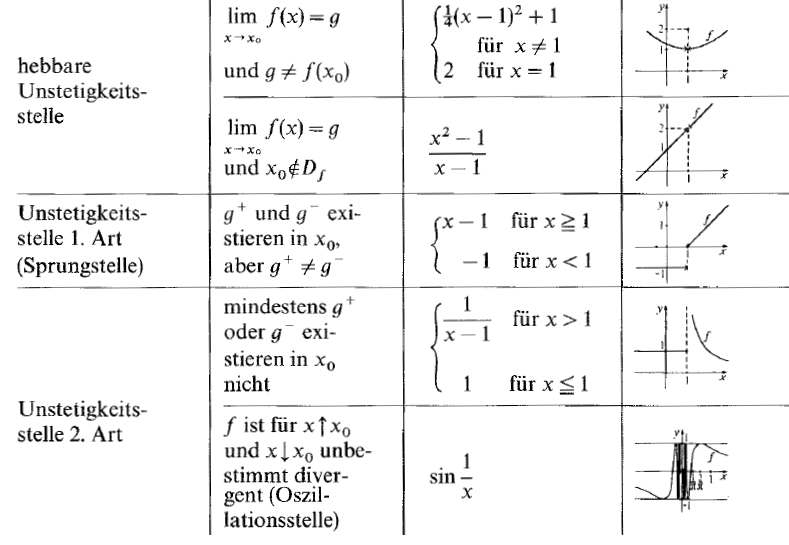
\includegraphics[width=\columnwidth]{./Images/unstetigkeit.png}

\subsubsection{Symmetrien}
\begin{tabular}{lll}
	\textbf{gerade}:& $f(-x) = f(x)$ & y-Symmetrisch\\
	\textbf{ungerade}:& $f(-x) = -f(x)$ & Nullpunkt-Symmetrisch\\
	\textbf{periodisch}:& $f(x) = f(x \pm p)$& Periode \\
\end{tabular}

\subsubsection{Monotonie}
Beschreibt das Wachstumsverhalten einer Reihe.\\
\noindent
\begin{tabular}{ll}
	\textbf{Wachsend $\Uparrow$ oder $\uparrow$}:& $a_{n+1} > a_n \Rightarrow a_{n+1} - a_n > 0$\\
	\textbf{Fallend $\Downarrow$ oder $\downarrow$}:& $a_{n+1} < a_n \Rightarrow a_{n+1} - a_n < 0$\\
\end{tabular}\\ \\

\noindent Die Monotonie einer Funktion kann durch die n-te Ableitung bestimmt werden.\\
\noindent\begin{tabular}{ll}
	$f \Uparrow$ & $f' > 0$\\
	$f \uparrow$ & $f' \geq 0$\\
	$f \Downarrow$ & $f' < 0$\\
	$f \downarrow$ & $f' \leq 0$\\
\end{tabular}

\subsubsection{Beschränktheit}
Eine Funktion ist beschränkt, wenn sie ein Infimum $k$ (Grösster unterer Wert) oder Supremum $K$ (Kleinster oberer Wert) Schranke hat. Das bedeutet $k < f(x) < K$

\subsubsection{Konvergenz / Divergenz}
Eine Funktion/Reihe ist \textbf{Konvergent}, wenn sie Beschränkt + Monoton ist, andern falls ist sie \textbf{Divergent}.
Konvergenz bestimmen:
\begin{enumerate}[nosep]
	\item Grenzwert berechnen (unter Vorbehalt)
	\item Monotonie prüfen (\underline{Hinweis}: \verweiseref{einschliessungsprinzip}, \verweiseref{bolzano}, \verweiseref{induktion})
	\item Beschränktheit prüfen anhand der Monotonie
\end{enumerate}

\subsubsection{Konvexität / Wendepunkt \bronstein{253}}
Auch als Krümmungsverhalten bekannt.\\
\begin{minipage}{\textwidth}	
	\begin{minipage}{0.2\textwidth}
		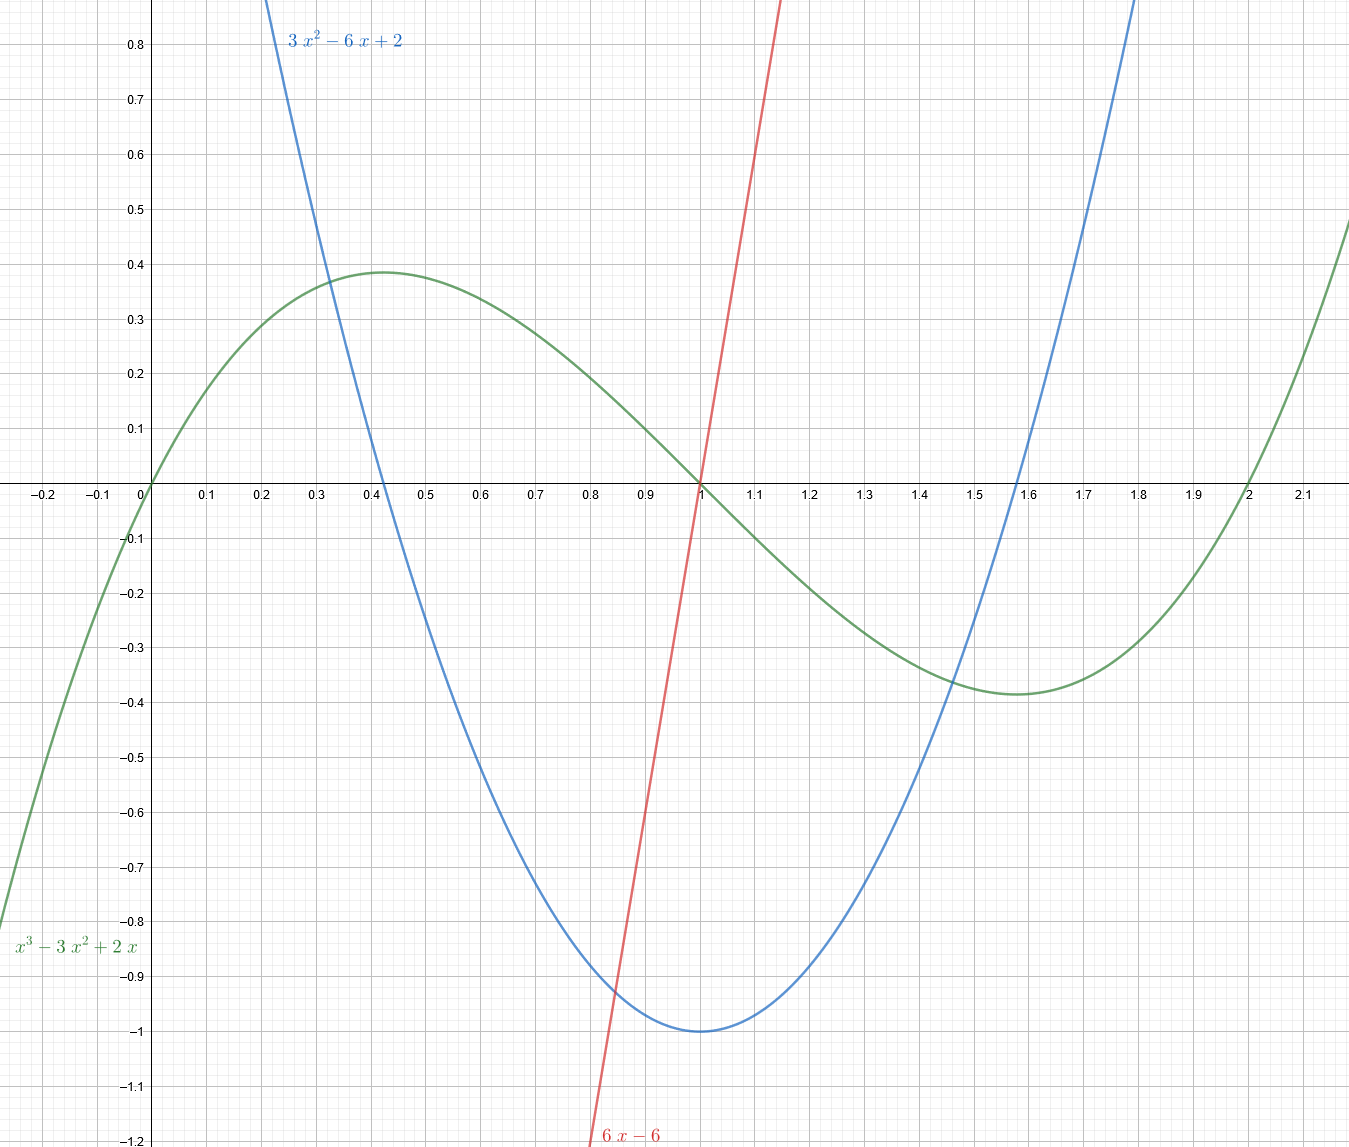
\includegraphics[width=\linewidth,keepaspectratio=true]{./Images/konvexkonkav.png}
	\end{minipage}%%% to prevent a space
	\begin{minipage}{0.3\textwidth}	
		\begin{itemize}[nosep]
			\item \textbf{Konvex} (Links Kurve):\\ $f'' > 0$ 
			\item \textbf{Streng Konvex} (Links Kurve):\\ $f'' \geq 0$ 
			
			\item \textbf{Konkav} (Rechts Kurve):\\ $f'' < 0$ 
			\item \textbf{Streng Konkav} (Rechts Kurve):\\ $f'' \leq 0$ 
			
			\item \textbf{Wendepunkt}:\\ Extremstelle 1.Ableitung, oder $f'' = 0$
		\end{itemize}
	\end{minipage}
\end{minipage}

\subsubsection{Asymptote \bronstein{259}}
Annähernde Kurve in 3 Typen (ZG: Zähler-Grad, NG: Nenner-Grad):\\
\begin{tabular}{p{1.5cm}p{3.1cm}p{4.2cm}}
	ZG $<$ NG & & $\frac{x}{x^2 - 4} \Rightarrow y = 0$ \\
	ZG $=$ NG & Quotient aus Koeffizienten von grössten Grad. & $\frac{2x-6}{x+4} \Rightarrow y = \frac{2}{1}$ \\
	ZG $>$ NG & Polynomdivision & $\frac{x^2 + 2x + 1}{x - 1} \Rightarrow \underbrace{x + 3}_{Asymptote} + \frac{4}{x -1}$
\end{tabular}

\subsection{Schnittwinkel}
Schnittwinkel zwischen zwei Geraden ($m: \text{Steigung} = f'(x)$):
\[ \tan(\alpha) = \frac{m_1 - m_2}{1 + m_1m_2} \]

\noindent Für Schnittwinkel $\alpha$ an Y-Achse, $g(x) = 0$ verwenden und Winkel $\beta$ an X-Achse berechnen. Anschliessend $90-\beta = \alpha$ rechnen.\\


\subsection{Nullstellen}
\noindent abc-Formel $x_{1,2} = \frac{-b\pm\sqrt{b^2-4ac}}{2a}$

\noindent Horner-Schema \\
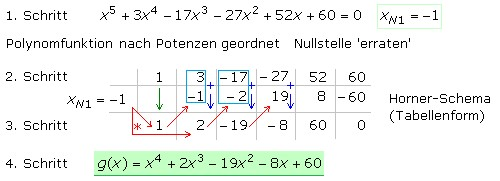
\includegraphics[width=\columnwidth]{./Images/horner.jpg}


\subsection{Partialbruchzerlegung \bronstein{15}}
\todo{TODO}

\subsection{Trigonometrisch}
\begin{center}
$ \text{rad} = \frac{\pi}{180°} \cdot \text{deg} \quad;\quad \text{deg} = \frac{180}{\pi} \cdot \text{rad} $
\end{center}

\begin{table}[ht]
	\centering
	\begin{tabular}{c|c|c|c|c|c|c|c|c|c}
		\rowcolor{LightGray}
		$\alpha$  & 0 & $\frac{\pi}{6}$ & $\frac{\pi}{4}$ & $\frac{\pi}{3}$ & $\frac{\pi}{2}$ & $\frac{2\pi}{3}$ & $\frac{3\pi}{4}$ & $\frac{5\pi}{6}$ & $\pi$ \\
		\rowcolor{LightGray}
		\tiny{$\alpha$°} & \tiny{0} & \tiny{30} & \tiny{45} & \tiny{60} & \tiny{90} & \tiny{120} & \tiny{135} & \tiny{150} & \tiny{180} \\
		\Xhline{2\arrayrulewidth}

		$\sin\alpha$ & 0 & $\frac{1}{2}$ & $\frac{\sqrt{2}}{2}$ & $\frac{\sqrt{3}}{2}$ & 1 & $\frac{\sqrt{3}}{2}$ & $\frac{\sqrt{2}}{2}$ & $\frac{1}{2}$ & 0 \\
		\hline
		$\cos\alpha$ & 1 & $\frac{\sqrt{3}}{2}$ & $\frac{\sqrt{2}}{2}$ & $\frac{1}{2}$ & 0 & -$\frac{1}{2}$ & $\frac{\sqrt{2}}{2}$ & $\frac{\sqrt{3}}{2}$ & -1 \\
		\hline
		$\tan\alpha$ & 0 & $\frac{1}{\sqrt{3}}$ & 1 & $\sqrt{3}$ & / & -$\sqrt{3}$ & -1 & -$\frac{1}{\sqrt{3}}$ & 0
	\end{tabular}
	\begin{tabular}{c|c|c|c|c|c|c|c|c}
		\rowcolor{LightGray}
		$\alpha$  & $\frac{7\pi}{6}$ & $\frac{5\pi}{4}$ & $\frac{4\pi}{3}$ & $\frac{3\pi}{2}$ & $\frac{5\pi}{3}$ & $\frac{7\pi}{4}$ & $\frac{11\pi}{6}$ & $2\pi$ \\
		\rowcolor{LightGray}
		\tiny{$\alpha$°} & \tiny{210} & \tiny{225} & \tiny{240} & \tiny{270} & \tiny{300} & \tiny{315} & \tiny{330} & \tiny{360} \\
		\Xhline{2\arrayrulewidth}
		
		$\sin\alpha$ & -$\frac{1}{2}$ & -$\frac{\sqrt{2}}{2}$ & -$\frac{\sqrt{3}}{2}$ & -1 & -$\frac{\sqrt{3}}{2}$ & -$\frac{\sqrt{2}}{2}$ & -$\frac{1}{2}$ & 0 \\
		\hline
		$\cos\alpha$ & -$\frac{\sqrt{3}}{2}$ & -$\frac{\sqrt{2}}{2}$ & -$\frac{1}{2}$ & 0 & $\frac{1}{2}$ & $\frac{\sqrt{2}}{2}$ & $\frac{\sqrt{3}}{2}$ & 1  \\
		\hline
		$\tan\alpha$ & $\frac{1}{\sqrt{3}}$ & 1 & $\sqrt{3}$ & / & -$\sqrt{3}$ & -1 & -$\frac{1}{\sqrt{3}}$ & 0
	\end{tabular}
\end{table}

\noindent Beziehungen:\\
\begin{tabular}{>{\(}l<{\)} @{\(\;=\;\)} >{\(}r<{\)}   >{\(}l<{\)} @{\(\;=\;\)} >{\(}r<{\)} }
	\cos(\alpha + 2\pi) & \cos(\alpha) & \sin(\alpha + 2\pi) & \sin(\alpha) \\
	\cos(-\alpha)                & \cos(\alpha)  & \sin(-\alpha)                & -\sin(\alpha) \\
	\cos(\pi - \alpha)           & -\cos(\alpha) & \sin(\pi - \alpha)           & \sin(\alpha)  \\
	\cos(\frac{\pi}{2} - \alpha) & \sin(\alpha)  & \sin(\frac{\pi}{2} - \alpha) & \cos(\alpha) \\
	\midrule
\end{tabular}
\begin{align*}
	1 &= \cos^2(\alpha) + \sin^2(\alpha) \\
	\midrule
	\sin(\alpha \pm \beta) &= \sin(\alpha)\cos(\beta) \pm \cos(\alpha)\sin(\beta) \\
	\cos(\alpha \pm \beta) &= \cos(\alpha)\cos(\beta) \mp \sin(\alpha)\sin(\beta) \\
	\tan\alpha \pm \beta &= \frac{\tan(\alpha)\cdot\tan(\beta)}{1\mp\tan(\alpha)\cdot\tan(\beta)} \\
	\midrule
	1 &= \cosh^2(\alpha) - \sinh^2(\alpha) \\
	\sinh(\alpha) &= \frac{e^\alpha - e^{-\alpha}}{2}\\
	\cosh(\alpha) &= \frac{e^\alpha + e^{-\alpha}}{2}\\
	\arcsinh(\alpha) &= \ln(\alpha + \sqrt{\alpha^2 - 1})\\
	\arccosh(\alpha) &= \ln(\alpha + \sqrt{\alpha^2 + 1})\\
	\midrule
	e^1 &= e \quad ln(1) = 0 \quad \ln(e^x) = x
\end{align*}



\section{Grenzwert}
\subsection{Formen}
\noindent\textbf{Bestimmt}
\begin{align*}
	\frac{g}{\infty} = 0,\; 
	\infty^\infty = \infty,\; 
	\frac{\infty}{0^\pm} = \pm\infty,\;
	\frac{1}{0^\pm} = \pm\infty,\;
	\\
	\frac{g}{0^+} = \begin{cases} \infty & g > 0\\-\infty & g < 0 \end{cases},\;
	\frac{\infty}{g} = \begin{cases} \infty & g > 0\\-\infty & g < 0 \end{cases}
\end{align*}

\noindent\textbf{Unbestimmt}
\begin{align*}
	\frac{0}{0},\;
	\frac{\infty}{\infty},\;
	0\cdot\infty,\;
	\infty - \infty,\;
	0^0,\; \infty^0,\;
	1^\infty
\end{align*}
siehe \verweiseref{lhopital} für die Bestimmung von \textit{unbestimmten} Grenzwerten

\subsection{Einschliessungs-Prinzip \bronstein{56}}\label{einschliessungsprinzip}
Wenn eine Funktionen $f(x)$ in $a(x) < f(x) < b(x)$ geschlossen ist, und wenn $\lim\limits_{x \rightarrow g}a(x) = G$ sowie $\lim\limits_{x \rightarrow g}b(x) = G$, dann ist auch $\lim\limits_{x \rightarrow g}f(x) = G$.

\subsection{Bolzano-Weierstrass}\label{bolzano}
Wenn eine Folge \underline{monoton} (Siehe \verweiseref{monotonie}) \textbf{und} \underline{beschränkt} (Siehe \verweiseref{beschränkt}) ist, dann ist diese auch Konvergent. Hinweis: Grenzwertgleichung alle $z_n$ durch $g$ ersetzten und nach $g$ Auflösen, $g$ muss im Intervall liegen!

\[
\left.\begin{aligned}
	\exists\sup f(x) &\text{ und } f(x) \Uparrow \\
	\exists\inf f(x) &\text{ und } f(x) \Downarrow
\end{aligned}
\right\rbrace \Rightarrow 
f(x) \text{konvergent}
\]

\noindent Supremum: kleinste obere Schranke, Infimum: grösste untere Schranke

\subsection{Bemerkenswerte Grenzwerte}
\begin{align*}
	\setlength\extrarowheight{8pt}
	\begin{array}{*2{>{\displaystyle}l}}
		\lim_{x\to 0} \frac{\sin x}{x} = 1 & \lim_{x\to\infty} \left(1 + \frac{\textcolor{red}{\pm a}}{x}\right)^x = e^{\textcolor{red}{\pm a}\texttt{}} \\
		\lim_{x\to 0} \frac{a^x - 1}{x} = \ln a & \lim_{x\to\infty} \frac{(\ln x)^a}{x^b} = 0 \\
		\lim_{x\to 0} \frac{e^x - 1}{2} = 0 & \lim_{x\to\infty} \sqrt[x]{p} = 1\\
		\lim_{x\to 0} x \cdot \ln x = 0 & \lim_{x\to\infty} \sum_{k=0}^x q^k = \frac{1}{1-q} \quad (|q| < 1)\\
	\end{array}
\end{align*}

\subsection{Bernoulli-l’Hôpital \bronstein{57}}\label{lhopital}
Wenn $\frac{f(x)}{g(x)} = \frac{0}{0}$ oder $\frac{\pm\infty}{\pm\infty}$ und $g'(x) \neq 0$ dann gilt:
\[
\lim\limits_{x \rightarrow a}\frac{f(x)}{g(x)} = \lim\limits_{x \rightarrow a}\frac{f'(x)}{g'(x)}
\]
Falls die Ableitung noch unbestimmt ist, einfach Wiederholen.
\newpage
\noindent\textbf{Hinweis}\\
\begin{tabular}{rrl}
	$f \cdot g\rightarrow $ & $ (0+) \cdot \infty$: & $\frac{f}{1 / g}$ vom Type $\frac{0}{0}$; $\frac{1/f}{g}$ vom Type $\frac{\infty}{\infty}$ \\ && \\
	$f - g \rightarrow $& $\infty - \infty$: & $\frac{1/g-1/f}{1/(f\cdot g)}$ vom Type $\frac{0}{0}$ \\ && \\
	$f^z \rightarrow$ & $ (0+)^0, \infty^0, 1^\infty$: & $e^{z\cdot\ln f}$
\end{tabular}\\ \\ 
Durch Ausklammern von Vorzeichen und Reziprokbildung bei negativen Exponenten sind andere Vorzeichenvarianten vollständig abgedeckt.

\section{Differenzialrechnungen}
\subsection{Differenzierbarkeit}
Beide $f'_1$ und $f'_-$ müssen existieren und gleich sind.
\[ \lim\limits_{h \rightarrow 0^+} \frac{f(x + h) - f(x)}{h} \eqi \lim\limits_{h \rightarrow 0^-} \frac{f(x + h) - f(x)}{h} \]

\subsubsection{Differential}\label{differential}
Das Differential ist $dy = f'(x) \cdot dx$ und kann mit $\underbrace{f(x) - f(x_0)}_\text{dy} = f'(x_0) \cdot \underbrace{(x - x_0)}_\text{dx}$ berechnet werden. (Siehe \bronstein{444})

\subsection{Ableitungsregeln \bronstein{446}}


{\setlength{\extrarowheight}{4pt}
\begin{tabular}{@{}lcl@{}}
	\textbf{f(x)} & $\rightarrow$ & \textbf{f'(x)} \\
	\toprule
	$c$ & $\rightarrow$ & $0$ \\
	$x^n$  & $\rightarrow$ & $n\cdot x^{n-1}$ \\
	$c\cdot g\left(x\right)$  & $\rightarrow$ & $c\cdot g'\left(x\right)$ \\
	$e^x$  & $\rightarrow$ & $e^x$ \\
	\midrule
	$g\left(x\right)+h\left(x\right)$  & $\rightarrow$ & $g'\left(x\right)+h'\left(x\right)$ \\
	$u\left(x\right)\cdot v\left(x\right)$  & $\rightarrow$ & $u'\left(x\right)\cdot v\left(x\right)+u\left(x\right)\cdot v'\left(x\right)$ \\ 
	$\frac{u\left(x\right)}{v\left(x\right)}$  & $\rightarrow$ & $\frac{u'\left(x\right)\cdot v\left(x\right)-u\left(x\right)\cdot v'\left(x\right)}{v^2\left(x\right)}$ \\
	$u\left(v\left(x\right)\right)$  & $\rightarrow$ & $u'\left(v\left(x\right)\right)\cdot v'\left(x\right)$ \\
	\midrule
	$\cos\left(x\right)$ & $\rightarrow$ & $-\sin(x)$ \\
	$\sin\left(x\right)$ & $\rightarrow$ & $\cos(x)$ \\	
	$\cosh\left(x\right)$ & $\rightarrow$ & $\sinh(x)$ \\
	$\sinh\left(x\right)$ & $\rightarrow$ & $\cosh(x)$ \\
	$\tan\left(x\right)$ & $\rightarrow$ & $\frac{1}{\cos^2(x)} = 1 + \tan^2(x)$ \\	
	$\ln\left(x\right)$ & $\rightarrow$ & $\frac{1}{x}$ \\
	$f^{-1}\left(x\right) {\scriptscriptstyle (Umkehrf.)}$  & $\rightarrow$ & $\frac{1}{f'(f^{-1}(x))}$ \\
	$\left|x\right|$ & $\rightarrow$ & $\frac{\left|x\right|}{x}$ \\
\end{tabular}
}


\subsection{Taylor-Reihe \bronstein{484}}
Das Tayler-Polynom approximiert eine Funktion um einen Entwicklungspunkt $a$:
\begin{align*}
	Tn(x, a) &= \sum\limits_{k = 0}^{n}\frac{f^{(k)}(a)}{k!}(x - a)^k \underbrace{+ R_n}_{\text{Restglied}}\\
	         &= f(a) + \frac{f'(a)}{1!}(x - a)^1 + \frac{f''(a)}{2!}(x - a)^2 + \dots
\end{align*}

\subsubsection{Linearisierung}
Spezialfall von Tayler-Polynom mit Entwicklungspunkt $a$:
\[Tn_2(x, a) = \hat{f}(x) = f(a) + f'(a)\cdot(x - a)\]

\subsubsection{Restglied}
\begin{tabular}{ll}
	Lagrange $R_n$ &= $\frac{f^{n + 1}(\xi)}{(n + 1)!} \cdot (x - a)^{n+1}$\\
	Couchy $R_n$ &= $\frac{f^{n + 1}(\xi)}{n!} \cdot (x - a)^{n+1} (1 - \beta)^n$
\end{tabular}


\subsubsection{Fehlerabschätzung}
\textbf{Absoluter}-Fehler: Maximum von gegebenem Intervall $I$ in $\left|R_n(x)\right|$ ($x \in I$) einsetzen. Achtung: Maximum variiert ja nach Funktion $f(x)$! Für $\xi \in [x, a]$ muss auch das Maximum gewählt werden, jedoch nur im Intervall von Entwicklungspunkt $a$ und gewähltem $x$.\\

\noindent Eine Funktion kann durch $R_n(x) = f(x) - T_n(x)$ gefunden werden.\\

\noindent\textbf{Relativer}-Fehler: $r = \frac{\text{absolut}}{f(x)} \rightarrow [\%]$

\subsection{Fehlerrechnung und Fortpflanzung}
\begin{center}
	\begin{tabular}{c|c|c|}
		\diagbox{Y}{X} & $\Delta x$ (Abs) & $\frac{\Delta x}{x}$ (Rel) \\
		\midrule
		$\Delta y$ (Abs) & A & B \\
		\midrule
		$\frac{\Delta y}{y}$ (Rel) & C & D
	\end{tabular}
\end{center}

\noindent Je nach Aufgabentype entsprechenden Fall in Tabelle wählen und von Y zu X rechnen. $\Delta x$ und $\Delta y$ müssen durch substituieren von \verweiseref{differential} ersetzt werden!

\noindent\textbf{Beispiel}: Rel.Y zu Rel.X rechnen (Fall D)
\[
\dfrac{dy}{y_0} \approxeq \dfrac{f'(x)dx}{y_0} \xRightarrow[Ziel]{}\dfrac{dx}{x}
\]

\subsubsection{Mittelwertsatz Differentialrechnung}
Der MWS \bronstein{454} wird oft für den Beweis einer Ungleichung verwendet, wenn die Funktion stetig und differenzierbar ist.
\begin{minipage}{\textwidth}	
	\begin{minipage}{0.2\textwidth}
		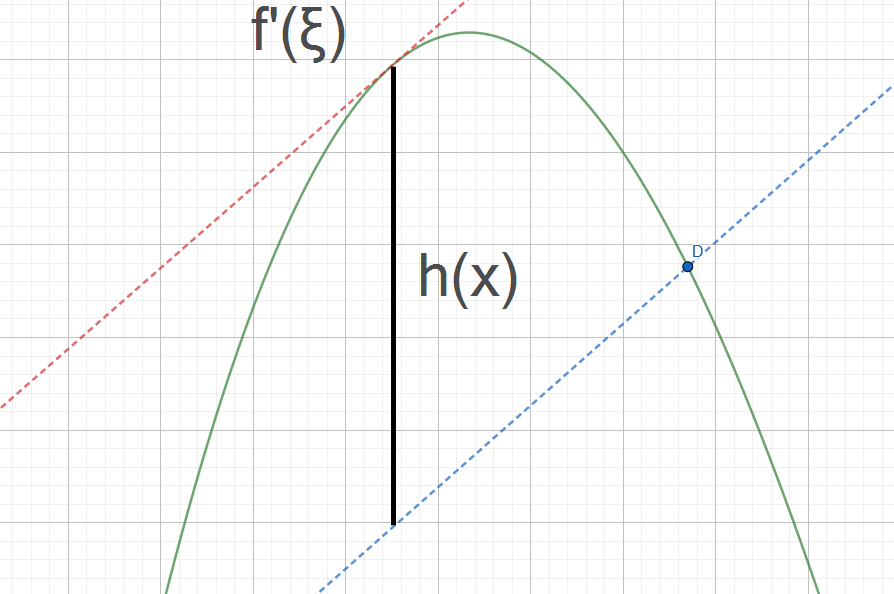
\includegraphics[width=\linewidth,keepaspectratio=true]{./Images/Mittelwertsatz.png}
	\end{minipage}%%% to prevent a space
	\begin{minipage}{0.3\textwidth}	
		\[f'(\xi) = \frac{f(b) - f(a)}{b - a}\] 
		\[ h(x) = \textcolor{green}{f(x)} - \textcolor{blue}{s(x)} \]
	\end{minipage}
\end{minipage}

\noindent\textbf{Beispiel} $\colorboxed{red}{\sin(x) < x},\quad x \in (0, \frac{\pi}{2}),\quad \xi \in (0, x)$
\[\xRightarrow{\text{MWS}} \sin'(\xi) = \cos(\xi) = \frac{\sin(x) - \sin(0)}{x - 0}\]
Weil $\xi$ zwischen 0 und $\frac{\pi}{2}$ ist, muss folgendes gelten: 

$
0 < \overbrace{\cos(\xi)}^{\text{MWS}} < 1 \rightarrow 0 < \frac{\sin(x)}{x} < 1 \rightarrow 0 < \colorboxed{red}{\sin(x) < x}
$


\subsection{Extremalwerte}
Um ein relative Extremalwert zu berechnen, muss die Steigung an $x_0 = 0$ sein:
$ f'(x_0) = 0 $ 
\noindent
Ob dieser Punkt nun ein Max,Min oder Sattelpunkt ist, kann die n-te Ableitung berechnet werden. \\Für \textbf{n-te Ableitung} Gerade ($2,3,\dots$) stimmt folgendes:
\[f^{(n)}(x_0) = \left\lbrace   \begin{array}{r@{}l}
	< 0 &\quad \text{Berg/relative. Maximum} \\
	> 0 &\quad \text{Tal/relative. Minimum} \\
	= 0 &\quad \text{Sattelpunkt oder \textbf{nächste Ableitung}!}
\end{array}\right.
\]
Wenn \textbf{n Ungerade} ($3, 5, \dots$) ist es ein Sattelpunkt. Falls auch $0$, nächste Ableitung



\section{Integralrechnung}
Das Riemann Integral zerlegt die Funktion $f$ in \textit{unendlich} viele Rechtecke mit Breite \textit{0} und einer zufälligen Höhe $\xi_i$. Die Summe aller Rechtecke konvergiert gegen die Fläche unter der Funktionslinie (Das Integral $I$).
\[
\int\limits_{a \text{ \tiny(untere Grenze)}}^{b \text{ \tiny(obere Grenze)}}f(x)dx = \lim_{\substack{n\to\infty\\\Delta x_i\to 0}} \sum\limits_{i = 1}^{n}f(\xi_i)\underbrace{(x_i - x_{i-1})}_{\Delta x_i}
\]
\noindent Eine Funktion $f$ ist Riemann integrierbar, wenn sie stetig oder monoton beschränkt und an höchstens endlich vielen Stellen unstetig ist.

\subsection{Bestimmtes Integral}
\[\int_{a}^{b}f(x)dx = F(b) - F(a) = \int_{a}^{0}f(x)dx + \int_{0}^{b}f(x)dx\]

\subsection{Formeln}
\noindent Flächeninhalt: \[A = \int_{a}^{b}\left|f(x)\right|dx\]
\noindent Integral Ableitung mit Funktion-Limits: \[\left(\int_{a(x)}^{b(x)}f(t)dt\right)' = f(b(x))b'(x) - f(a(x))a'(x)\]
\noindent Integral Ungleichung:
\[\left|\int_{a}^{b}f(x)dx\right| \leq \int_{a}^{b}\left|f(x)\right|dx\]

\subsection{Mittelwertsatz Integral}
Sei $f(x)$ in $[a;b]$ stetig, dann ist der Mittelwert (RMS) aller Punkte:
\[\frac{1}{b-a}\int_{a}^{b}f(x)dx\]




% To save some space, it's not printed on PDF
% \begin{thebibliography}{1}
%	\bibitem{hsr}
%	\texttt{An1E} Vorlesungen an der OST Rapperswil und dem dazugehörigen Skript,
%	\textit{Dr. Bernhard Zgraggen}, Herbstsemester 2020
%	\bibitem{bronstein}
%	Taschenbuch der Mathematik,
%	11. \"uberarbeitete Auflage, 2020 (1977),
%	\textit{Bronstein, Semendjajew, Musiol, M\"uhlig}, 
%	\texttt{ISBN 978-3-8085-5792-1}
% \end{thebibliography}

\end{document}